


\chapter{Conditionals and recursion  |  条件和递归}

The main topic of this chapter is the {\tt if} statement, which
executes different code depending on the state of the program.
But first I want to introduce two new operators: floor division
and modulus.

这章的中心话题是能够根据程序的状态执行不同命令的 if 语句。但是首先我想介绍两个新的运算符 : {\em 地板除法} (floor division) \footnote{译注:向下取整的除法。} 和{\em 求余} (modulus) 。

\section{Floor division and modulus  |  地板除法和求余}

The {\bf floor division} operator, \verb"//", divides
two numbers and rounds down to an integer.  For example, suppose the
run time of a movie is 105 minutes.  You might want to know how
long that is in hours.  Conventional division
returns a floating-point number:

{\em 地板除运算符} (floor division operator)为 \li{//} 即先做除法,然后将结果向下保留到整数。 例如,如果一部电影时长105 分钟,你可能想知道这代表着多少小时。 传统的除法操作会返回一个浮点数:

\begin{lstlisting}
>>> minutes = 105
>>> minutes / 60
1.75
\end{lstlisting}

But we don't normally write hours with decimal points.  Floor
division returns the integer number of hours, dropping the
fraction part:

但是,以小时做单位时我们通常不会写出小数部分。地板除法丢弃除法运算结果的小数部分,返回整数个小时:

\begin{lstlisting}
>>> minutes = 105
>>> hours = minutes // 60
>>> hours
1
\end{lstlisting}

To get the remainder, you could subtract off one hour in minutes:

如果你希望得到余数,你可以从除数中减去一个小时也就是 60 分钟:

\begin{lstlisting}
>>> remainder = minutes - hours * 60
>>> remainder
45
\end{lstlisting}

\index{floor division}  \index{floating-point division}
\index{division!floor}  \index{division!floating-point}
\index{modulus operator}  \index{operator!modulus}

An alternative is to use the {\bf modulus operator}, \verb"%", which
divides two numbers and returns the remainder.

另一个方法就是使用 {\em 求余运算符} (modulus operator), \li{%} ,它会将两个数相除,返回余数。


\begin{lstlisting}
>>> remainder = minutes % 60
>>> remainder
45
\end{lstlisting}

%
The modulus operator is more useful than it seems.  For
example, you can check whether one number is divisible by another---if
{\tt x \% y} is zero, then {\tt x} is divisible by {\tt y}.

求余运算符比看起来更加有用。例如,你可以查看一个数是否可以被另一个数整除——如果 \li{x % y} 的结果是 $0$,那么 \li{x} 能被 \li{y} 整除。
\index{divisibility}

Also, you can extract the right-most digit
or digits from a number.  For example, {\tt x \% 10} yields the
right-most digit of {\tt x} (in base 10).  Similarly {\tt x \% 100}
yields the last two digits.

此外,你也能获得一个数的最右边一位或多位的数字。 例如, \li{x % 10} 返回 \li{x} 最右边一位的数字(十进制)。 类似地,\li{x % 100} 返回最后两位数字。

If you are using Python 2, division works differently.  The
division operator, \verb"/", performs floor division if both
operands are integers, and floating-point division if either
operand is a {\tt float}.

如果你正在使用 Python 2, 那么除法就会和前面的介绍有点不同。除法运算符 \li{/} 在被除数和除数都是整数的时候,会进行地板除,但是当被除数和除数中任意一个是浮点数的时候,则进行浮点数除法。\footnote{译注:在 Python3 中,无论任何类型都会保持小数部分。}
\index{Python 2}


\section{Boolean expressions  |  布尔表达式}
\index{boolean expression}  \index{expression!boolean}
\index{logical operator}  \index{operator!logical}

A {\bf boolean expression} is an expression that is either true
or false.  The following examples use the
operator {\tt ==}, which compares two operands and produces
{\tt True} if they are equal and {\tt False} otherwise:

{\em 布尔表达式} (boolean expression) 的结果要么为真要么为假。
下面的例子使用 \li{==} 运算符。它比较两个运算数,
如果它们相等,则结果为 \li{True} ,否则结果为 \li{False} 。

\begin{lstlisting}
>>> 5 == 5
True
>>> 5 == 6
False
\end{lstlisting}

%
{\tt True} and {\tt False} are special
values that belong to the type {\tt bool}; they are not strings:

\li{True} 和 \li{False} 是属于bool类型的特殊值;它们不是字符串。
\index{True special value}  \index{False special value}
\index{special value!True}  \index{special value!False}
\index{bool type}  \index{type!bool}

\begin{lstlisting}
>>> type(True)
<class 'bool'>
>>> type(False)
<class 'bool'>
\end{lstlisting}

%
The {\tt ==} operator is one of the {\bf relational operators}; the
others are:

\li{==} 运算符是 {\em 关系运算符} (relational operators) 之一; 其他关系运算符还有:


\begin{lstlisting}
      x != y               # x is not equal to y
      x > y                # x is greater than y
      x < y                # x is less than y
      x >= y               # x is greater than or equal to y
      x <= y               # x is less than or equal to y
\end{lstlisting}

%
Although these operations are probably familiar to you, the Python
symbols are different from the mathematical symbols.  A common error
is to use a single equal sign ({\tt =}) instead of a double equal sign
({\tt ==}).  Remember that {\tt =} is an assignment operator and
{\tt ==} is a relational operator.   There is no such thing as
{\tt =<} or {\tt =>}.

虽然这些运算符对你来说可能很熟悉,但是 Python 的符号与数学符号不相同。
一个常见的错误是使用单独一个等号 (\li{=}) 而不是双等号 (\li{==})。
请记住, \li{=} 是赋值运算符, \li{==} 是关系运算符。 没有类似 \li{=<} 或 \li{=>} 的东西。

\index{relational operator}  \index{operator!relational}
\index{关系型运算符}  \index{运算符!关系型}

\section {Logical operators  |  逻辑运算符}
\index{logical operator}  \index{operator!logical}

There are three {\bf logical operators}: {\tt and}, {\tt
or}, and {\tt not}.  The semantics (meaning) of these operators is
similar to their meaning in English.  For example,
{\tt x > 0 and x < 10} is true only if {\tt x} is greater than 0
{\em and} less than 10.

有三个 {\em 逻辑运算符} (logical operators) : \li{and} 、 \li {or} 和 \li {not}。
这些运算符的含义和它们在英语的意思相似。例如, \li{x > 0 and x < 10} 只在 \li{x} 大于 \li{0} {\bf 并且} 小于 \li{10} 时为真。


\index{and operator}  \index{or operator}
\index{not operator}  \index{operator!and}
\index{operator!or}  \index{operator!not}

{\tt n\%2 == 0 or n\%3 == 0} is true if {\em either or both} of the
conditions is true, that is, if the number is divisible by 2 {\em or}
3.

\li{n%2 == 0 or n%3 == 0} 中如果 {\em 一个或两个} 条件为真,那么整个表达式即为真。也就是说,如果数字\li{n} 能被 \li{2} {\em 或者} \li{3} 整除,则为真。

Finally, the {\tt not} operator negates a boolean
expression, so {\tt not (x > y)} is true if {\tt x > y} is false,
that is, if {\tt x} is less than or equal to {\tt y}.

最后,\li{not} 运算符对一个布尔表达式取反, 因此,如果 \li{x > y} 为假,也就是说 \li{x} 小于或等于 \li{y}, 则 \li{not (x > y)} 为真。

Strictly speaking, the operands of the logical operators should be
boolean expressions, but Python is not very strict.
Any nonzero number is interpreted as {\tt True}:

严格来讲,逻辑运算符的运算数应该是布尔表达式,
但是Python并不严格要求。任何非0的数字都被解释成为真 ( \li{True} )。

\begin{lstlisting}
>>> 42 and True
True
\end{lstlisting}

%
This flexibility can be useful, but there are some subtleties to
it that might be confusing.  You might want to avoid it (unless
you know what you are doing).

这种灵活性很有用,但有一些细节可能容易令人困惑。你可能需要避免这种用法(除非你知道你正在做什么)。


\section{Conditional execution  |  有条件执行}
\label{conditional.execution}

\index{conditional statement}  \index{statement!conditional}
\index{if statement}  \index{statement!if}
\index{conditional execution}

In order to write useful programs, we almost always need the ability
to check conditions and change the behavior of the program
accordingly.  {\bf Conditional statements} give us this ability.  The
simplest form is the {\tt if} statement:

为了写出有用的程序,我们几乎总是需要能够检测条件,并相应地改变程序行为。
{\em 条件语句} (Conditional statements) 给予了我们这一能力。
最简单的形式是 \li{if} 语句:

\begin{lstlisting}
if x > 0:
    print('x is positive')
\end{lstlisting}

%
The boolean expression after {\tt if} is
called the {\bf condition}.  If it is true, the indented
statement runs.  If not, nothing happens.

\li{if} 之后的布尔表达式被称作 {\em 条件} (condition) 。
如果它为真,则缩进的语句会被执行。 如果不是,则什么也不会发生。
\index{condition}  \index{compound statement}
\index{statement!compound}

{\tt if} statements have the same structure as function definitions:
a header followed by an indented body.  Statements like this are
called {\bf compound statements}.

\li{if} 语句和函数定义有相同的结构:一个语句头跟着一个缩进的语句体。
类似的语句被称作 {\em 复合语句} (compound statements) 。

There is no limit on the number of statements that can appear in
the body, but there has to be at least one.
Occasionally, it is useful to have a body with no statements (usually
as a place keeper for code you haven't written yet).  In that
case, you can use the {\tt pass} statement, which does nothing.

语句体中可出现的语句数目没有限制,但是至少得有一个。
有时候,一条语句都没有的语句体也是有用的(通常是为你还没写的代码占一个位子)。
这种情况下,你可以使用 \li{pass} 语句,它什么也不做。
\index{pass statement}  \index{statement!pass}


\begin{lstlisting}
if x < 0:
    pass          # TODO: need to handle negative values!
\end{lstlisting}
%

\section{Alternative execution  |  二选一执行}
\label{alternative.execution}
\index{alternative execution}  \index{else keyword}  \index{keyword!else}

A second form of the {\tt if} statement is ``alternative execution'',
in which there are two possibilities and the condition determines
which one runs.  The syntax looks like this:

\li{if} 语句的第二种形式是 {\em ``二选一执行''} (alternative execution) ,
此时有两个可能的选择,由条件决定执行哪一个。 语法看起来是这样:


\begin{lstlisting}
if x % 2 == 0:
    print('x is even')
else:
    print('x is odd')
\end{lstlisting}
%
If the remainder when {\tt x} is divided by 2 is 0, then we know that
{\tt x} is even, and the program displays an appropriate message.  If
the condition is false, the second set of statements runs.
Since the condition must be true or false, exactly one of the
alternatives will run.  The alternatives are called {\bf
  branches}, because they are branches in the flow of execution.

如果 \li{x} 除以 \li{2} 的余数是 \li{0},那么我们知道 \li{x} 是偶数,
然后程序会打印相应的信息。 如果条件为假,则执行第二部分语句。
由于条件要么为真要么为假,两个选择中只有一个会被执行。
这些选择被称作\ **分支(branches)**\ ,因为它们是执行流程的分支。

\index{branch}  \index{分支}


\section{Chained conditionals  |  链式条件}
\index{chained conditional}  \index{conditional!chained}

Sometimes there are more than two possibilities and we need more than
two branches.  One way to express a computation like that is a {\bf
chained conditional}:

有时有超过两个可能的情况,于是我们需要多于两个的分支。
表示像这样的计算的方法之一是{\em 链式条件} (chained conditional):

\begin{lstlisting}
if x < y:
    print('x is less than y')
elif x > y:
    print('x is greater than y')
else:
    print('x and y are equal')
\end{lstlisting}
%
{\tt elif} is an abbreviation of ``else if''.  Again, exactly one
branch will run.  There is no limit on the number of {\tt
elif} statements.  If there is an {\tt else} clause, it has to be
at the end, but there doesn't have to be one.

\li{elif} 是 ``else if''的缩写。 同样地,这里只有一个分支会被执行。
\li{elif} 语句的数目没有限制。如果有一个 \li{else} 从句,
它必须是在最后,但这个语句并不是必须。
\index{elif keyword}  \index{keyword!elif}

\begin{lstlisting}
if choice == 'a':
    draw_a()
elif choice == 'b':
    draw_b()
elif choice == 'c':
    draw_c()
\end{lstlisting}

%
Each condition is checked in order.  If the first is false,
the next is checked, and so on.  If one of them is
true, the corresponding branch runs and the statement
ends.  Even if more than one condition is true, only the
first true branch runs.

程序将按顺序逐个检测条件,如果第一个为假,检测下一个,以此类推。
如果它们中有一个为真,相应的分支被执行,并且语句结束。
即便有不止一个条件为真,也只执行第一个为真的分支。

\section{Nested conditionals  |  嵌套条件}
\index{nested conditional}  \index{conditional!nested}

One conditional can also be nested within another.  We could have
written the example in the previous section like this:

一个条件可以嵌到另一个里面。我们可以这样写前一节的例子:

\begin{lstlisting}
if x == y:
    print('x and y are equal')
else:
    if x < y:
        print('x is less than y')
    else:
        print('x is greater than y')
\end{lstlisting}

%
The outer conditional contains two branches.  The
first branch contains a simple statement.  The second branch
contains another {\tt if} statement, which has two branches of its
own.  Those two branches are both simple statements,
although they could have been conditional statements as well.

外层的条件 (outer conditional) 包括两个分支。第一个分支包括一条简单的语句。
第二个分支又包括一个 \li{if} 语句,它有自己的两个分支。
那两个分支都是简单的语句,当然它们也可以是条件语句。


Although the indentation of the statements makes the structure
apparent, {\bf nested conditionals} become difficult to read very
quickly.  It is a good idea to avoid them when you can.

虽然语句的缩进使得结构很明显,但是仍然很难快速地阅读 {\em 嵌套条件} (nested conditionals) 。当你可以的时候,避免使用嵌套条件是个好办法。

Logical operators often provide a way to simplify nested conditional
statements.  For example, we can rewrite the following code using a
single conditional:

逻辑运算符通常是一个简化嵌套条件语句的方法。
例如,我们可以用一个单一条件重写下面的代码:

\begin{lstlisting}
if 0 < x:
    if x < 10:
        print('x is a positive single-digit number.')
\end{lstlisting}

%
The {\tt print} statement runs only if we make it past both
conditionals, so we can get the same effect with the {\tt and} operator:

只有通过了两个条件检测的时候, \li{print} 语句才被执行,
因此我们可以用 \li{and} 运算符得到相同的效果:


\begin{lstlisting}
if 0 < x and x < 10:
    print('x is a positive single-digit number.')
\end{lstlisting}

For this kind of condition, Python provides a more concise option:

对于这样的条件,Python 提供了一种更加简洁的写法。

\begin{lstlisting}
if 0 < x < 10:
    print('x is a positive single-digit number.')
\end{lstlisting}


\section{Recursion  |  递归}
\label{recursion}
\index{recursion}  \index{递归}

It is legal for one function to call another;
it is also legal for a function to call itself.  It may not be obvious
why that is a good thing, but it turns out to be one of the most
magical things a program can do.
For example, look at the following function:

一个函数调用另一个是合法的;一个函数调用它自己也是合法的。
这样的好处可能并不是那么明显,但它实际上成为了程序能做到的最神奇的事情之一。
例如,看一下这个程序:

\begin{lstlisting}
def countdown(n):
    if n <= 0:
        print('Blastoff!')
    else:
        print(n)
        countdown(n-1)
\end{lstlisting}

%
If {\tt n} is 0 or negative, it outputs the word, ``Blastoff!''
Otherwise, it outputs {\tt n} and then calls a function named {\tt
countdown}---itself---passing {\tt n-1} as an argument.

如果n是0或负数,程序输出单词 ``Blastoff!''。
否则,它输出n然后调用一个名为 \li{countdown} 的函数—即它自己 --- 传递 \li{n-1} 作为实参。

What happens if we call this function like this?

如果我们像这样调用该函数会发生什么呢?


\begin{lstlisting}
>>> countdown(3)
\end{lstlisting}

%
The execution of {\tt countdown} begins with {\tt n=3}, and since
{\tt n} is greater than 0, it outputs the value 3, and then calls itself...

\begin{quote}
The execution of {\tt countdown} begins with {\tt n=2}, and since
{\tt n} is greater than 0, it outputs the value 2, and then calls itself...

\begin{quote}
The execution of {\tt countdown} begins with {\tt n=1}, and since
{\tt n} is greater than 0, it outputs the value 1, and then calls itself...

\begin{quote}
The execution of {\tt countdown} begins with {\tt n=0}, and since {\tt
n} is not greater than 0, it outputs the word, ``Blastoff!'' and then
returns.
\end{quote}

The {\tt countdown} that got {\tt n=1} returns.
\end{quote}

The {\tt countdown} that got {\tt n=2} returns.
\end{quote}

The {\tt countdown} that got {\tt n=3} returns.

And then you're back in \verb"__main__".  So, the
total output looks like this:


\li{countdown} 开始以 \li{n=3} 执行,由于 \li{n} 大于 0, 它输出值 3,然后调用它自己...

\begin{quote}
\li{countdown} 开始以 \li{n=2} 执行,由于 \li{n} 大于 0, 它输出值 2,然后调用它自己...

\begin{quote}
\li{countdown} 开始以 \li{n=1} 执行,既然 \li{n} 大于 0,它输出值 1,然后调用它自己...

\begin{quote}
\li{countdown} 开始以 \li{n=0} 执行,由于 \li{n} 不大于 0, 它输出单词 ``Blastoff!'',然后返回。
\end{quote}

获得 \li{n=1} 的 \li{countdown} 返回。
\end{quote}

获得 \li{n=2} 的 \li{countdown} 返回。
\end{quote}

获得 \li{n=3} 的 \li{countdown} 返回。

然后回到 \li{__main__} 中。 因此整个输出类似于:

\begin{lstlisting}
3
2
1
Blastoff!
\end{lstlisting}

%
A function that calls itself is {\bf recursive}; the process of
executing it is called {\bf recursion}.

一个调用它自己的函数是 {\em 递归的} (recursive) ;
这个过程被称作 {\em 递归} (recursion) 。
\index{recursion}  \index{function!recursive}
\index{递归}  \index{函数!递归}

As another example, we can write a function that prints a
string {\tt n} times.

再举一例,我们可以写一个函数,其打印一个字符串 \li{n} 次。

\begin{lstlisting}
def print_n(s, n):
    if n <= 0:
        return
    print(s)
    print_n(s, n-1)
\end{lstlisting}

%
If {\tt n <= 0} the {\bf return statement} exits the function.  The
flow of execution immediately returns to the caller, and the remaining
lines of the function don't run.

如果 \li{n <= 0} ,\li{return}{\em 语句} 退出函数。
执行流程马上返回到调用者,函数剩余的语句行不会被执行。
\index{return statement}  \index{statement!return}

The rest of the function is similar to {\tt countdown}: it displays
{\tt s} and then calls itself to display {\tt s} $n-1$ additional
times.  So the number of lines of output is {\tt 1 + (n - 1)}, which
adds up to {\tt n}.

函数的其余部分和 \li{countdown} 相似: 它打印 \li{s} 的值,然后调用自身打印 \li{s} $n-1$ 次。 因此,输出的行数是 \li{1 + (n - 1)} ,加起来是 \li{n}。

For simple examples like this, it is probably easier to use a {\tt
for} loop.  But we will see examples later that are hard to write
with a {\tt for} loop and easy to write with recursion, so it is
good to start early.

对于像这样简单的例子,使用for循环可能更容易。
但是我们后面将看到一些用for循环很难写,用递归却很容易的例子,
所以早点儿开始学习递归有好处。
\index{for loop}  \index{loop!for}


\section{Stack diagrams for recursive functions  |  递归函数的堆栈图}
\label{recursive.stack}
\index{stack diagram}  \index{function frame}  \index{frame}

In Section~\ref{stackdiagram}, we used a stack diagram to represent
the state of a program during a function call.  The same kind of
diagram can help interpret a recursive function.

在 Section~\ref{stackdiagram} 一节中,我们用堆栈图表示了一个函数调用期间程序的状态。
这种图也能帮我们理解递归函数。

Every time a function gets called, Python creates a
frame to contain the function's local variables and parameters.
For a recursive function, there might be more than one frame on the
stack at the same time.

每当一个函数被调用时,Python 生成一个新的栈帧,用于保存函数的局部变量和形参。
对于一个递归函数,在堆栈上可能同时有多个栈帧。

Figure~\ref{fig.stack2} shows a stack diagram for {\tt countdown} called with
{\tt n = 3}.

图~\ref{fig.stack2} 展示了一个以 \li{n = 3} 调用 \li{countdown} 的堆栈图。

\begin{figure}
\centerline
{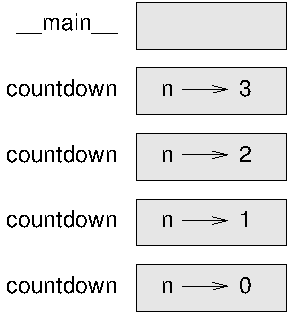
\includegraphics[scale=0.8]{../source/figs/stack2.pdf}}
\caption{Stack diagram.}
\label{fig.stack2}
\end{figure}


As usual, the top of the stack is the frame for \verb"__main__".
It is empty because we did not create any variables in
\verb"__main__" or pass any arguments to it.
\index{base case}  \index{recursion!base case}

通常,堆栈的顶部是 \li{__main__} 栈帧。
因为我们在 \li{__main__} 中没有创建任何变量,也没有传递任何实参给它,所以它是空的。

The four {\tt countdown} frames have different values for the
parameter {\tt n}.  The bottom of the stack, where {\tt n=0}, is
called the {\bf base case}.  It does not make a recursive call, so
there are no more frames.

对于形参 \li{n} ,四个 \li{countdown} 栈帧有不同的值。 \li{n=0} 的栈底,被称作 {\em 基础情形} (base case) 。
它不再进行递归调用了,所以没有更多的栈帧了。

As an exercise, draw a stack diagram for \verb"print_n" called with
\verb"s = 'Hello'" and {\tt n=2}.
Then write a function called \verb"do_n" that takes a function
object and a number, {\tt n}, as arguments, and that calls
the given function {\tt n} times.

接下来练习一下,请画一个以 \li{s = 'Hello'} 和 \li{n=2} 调用 \li{print_n} 的堆栈图。
写一个名为 \li{do_n} 的函数,接受一个函数对象和一个数 \li{n} 作为实参,
能够调用指定的函数 \li{n} 次。


\section{Infinite recursion  |  无限递归}
\index{infinite recursion}  \index{recursion!infinite}
\index{runtime error}  \index{error!runtime}
\index{traceback}

If a recursion never reaches a base case, it goes on making
recursive calls forever, and the program never terminates.  This is
known as {\bf infinite recursion}, and it is generally not
a good idea.  Here is a minimal program with an infinite recursion:

如果一个递归永不会到达基础情形,它将永远进行递归调用,
并且程序永远不会终止。这被称作 {\em 无限递归} (infinite recursion) ,
通常这不是一个好主意。下面是一个最简单的无限递归程序:

\begin{lstlisting}
def recurse():
    recurse()
\end{lstlisting}
%
In most programming environments, a program with infinite recursion
does not really run forever.  Python reports an error
message when the maximum recursion depth is reached:

在大多数编程环境里,一个具有无限递归的程序并非永远不会终止。
当达到最大递归深度时,Python会报告一个错误信息:
\index{exception!RuntimeError}  \index{RuntimeError}

\begin{lstlisting}
  File "<stdin>", line 2, in recurse
  File "<stdin>", line 2, in recurse
  File "<stdin>", line 2, in recurse
                  .
                  .
                  .
  File "<stdin>", line 2, in recurse
RuntimeError: Maximum recursion depth exceeded
\end{lstlisting}
%
This traceback is a little bigger than the one we saw in the
previous chapter.  When the error occurs, there are 1000
{\tt recurse} frames on the stack!

此回溯比我们在前面章节看到的长一些。
当错误出现的时候,在堆栈上有 1000 个{\em 递归栈帧}!

If you write encounter an infinite recursion by accident, review
your function to confirm that there is a base case that does not
make a recursive call.  And if there is a base case, check whether
you are guaranteed to reach it.

如果你不小心遇到了无限递归,检查你的函数,确保基础情形没有继续调用递归。
同时如果确实有基础情形,请检查基础情形是不是能够出现这种情形。

\section{Keyboard input  |  键盘输入}
\index{keyboard input}

The programs we have written so far accept no input from the user.
They just do the same thing every time.

到目前为止,我们所写的程序都不接受来自用户的输入。
每次它们都只是做相同的事情。

Python provides a built-in function called {\tt input} that
stops the program and
waits for the user to type something.  When the user presses {\sf
  Return} or {\sf Enter}, the program resumes and \verb"input"
returns what the user typed as a string.  In Python 2, the same
function is called \verb"raw_input".

Python 提供了一个内建函数 \li{input} ,可以暂停程序运行,并等待用户输入。
当用户按下回车键(Return or Enter),程序恢复执行,\li{input} 以字符串形式返回用户键入的内容。在 Python 2 中,这个函数的名字叫 \li{raw_input} 。
\index{Python 2}  \index{input function}  \index{function!input}

\begin{lstlisting}
>>> text = input()
What are you waiting for?
>>> text
What are you waiting for?
\end{lstlisting}
%
Before getting input from the user, it is a good idea to print a
prompt telling the user what to type.  \verb"input" can take a
prompt as an argument:

在从用户那儿获得输入之前,打印一个提示告诉用户输入什么是个好办法。
\li{input} 接受提示语作为实参。
\index{prompt}

\begin{lstlisting}
>>> name = input('What...is your name?\n')
What...is your name?
Arthur, King of the Britons!
>>> name
Arthur, King of the Britons!
\end{lstlisting}
%
The sequence \verb"\n" at the end of the prompt represents a {\bf
  newline}, which is a special character that causes a line break.
That's why the user's input appears below the prompt.  \index{newline}

提示语最后的 \li{\n} 表示一个 {\em 新行} (newline) ,
它是一个特别的字符,会造成换行。 这也是用户的输入出现在提示语下面的原因。

If you expect the user to type an integer, you can try to convert
the return value to {\tt int}:

如果你期望用户键入一个整型数,那么你可以试着将返回值转化为 \li{int} :

\begin{lstlisting}
>>> prompt = 'What...is the airspeed velocity of an unladen swallow?\n'
>>> speed = input(prompt)
What...is the airspeed velocity of an unladen swallow?
42
>>> int(speed)
42
\end{lstlisting}
%
But if the user types something other than a string of digits,
you get an error:

但是,如果用户输入不是数字构成的字符串,你会获得一个错误:

\begin{lstlisting}
>>> speed = input(prompt)
What...is the airspeed velocity of an unladen swallow?
What do you mean, an African or a European swallow?
>>> int(speed)
ValueError: invalid literal for int() with base 10
\end{lstlisting}

%
We will see how to handle this kind of error later.

我们后面将介绍处理这类错误的方法。
\index{ValueError}  \index{exception!ValueError}


\section{Debugging  |  调试}
\label{whitespace}
\index{debugging}  \index{traceback}

When a syntax or runtime error occurs, the error message contains
a lot of information, but it can be overwhelming.  The most
useful parts are usually:

当出现语法错误和运行时错误的时候,错误信息中会包含了很多的信息,但是信息量有可能太大。通常,最有用的部分是:

\begin{itemize}

\item What kind of error it was, and

\item Where it occurred.

\end{itemize}

\begin{itemize}

\item 是哪类错误,以及

\item 在哪儿出现。

\end{itemize}

Syntax errors are usually easy to find, but there are a few
gotchas.  Whitespace errors can be tricky because spaces and
tabs are invisible and we are used to ignoring them.

语法错误通常很容易被找到,但也有一些需要注意的地方。
空白分隔符错误很棘手,因为空格和制表符是不可见的,而且我们习惯于忽略它们。
\index{whitespace}

\begin{lstlisting}
>>> x = 5
>>>  y = 6
  File "<stdin>", line 1
    y = 6
    ^
IndentationError: unexpected indent
\end{lstlisting}

%
In this example, the problem is that the second line is indented by
one space.  But the error message points to {\tt y}, which is
misleading.  In general, error messages indicate where the problem was
discovered, but the actual error might be earlier in the code,
sometimes on a previous line.

在这个例子中,问题在于第二行缩进了一个空格。
但是错误信息指向y,这是个误导。 通常,错误信息指向发现错误的地方,
但是实际的错误可能发生在代码中更早的地方, 有时在前一行。
\index{error!runtime}  \index{runtime error}

The same is true of runtime errors.  Suppose you are trying
to compute a signal-to-noise ratio in decibels.  The formula
is $SNR_{db} = 10 \log_{10} (P_{signal} / P_{noise})$.  In Python,
you might write something like this:

运行时错误也同样存在这个问题。假设你正试图计算分贝信噪比。
公式是 $SNR_{db} = 10 \log_{10} (P_{signal} / P_{noise})$ 。
在 Python 中,你可能会写出这样的代码:

\begin{lstlisting}
import math
signal_power = 9
noise_power = 10
ratio = signal_power // noise_power
decibels = 10 * math.log10(ratio)
print(decibels)
\end{lstlisting}
%
When you run this program, you get an exception:

但是,当你运行它的时候, 你却获得一个异常。

%
\index{exception!OverflowError}  \index{OverflowError}

\begin{lstlisting}
Traceback (most recent call last):
  File "snr.py", line 5, in ?
    decibels = 10 * math.log10(ratio)
ValueError: math domain error
\end{lstlisting}
%
The error message indicates line 5, but there is nothing
wrong with that line.  To find the real error, it might be
useful to print the value of {\tt ratio}, which turns out to
be 0.  The problem is in line 4, which uses floor division
instead of floating-point division.

该错误信息指向第 5 行,但是那一行没什么错误。
为了找到真正的错误,打印 \li{ratio} 的值也许会有用,结果发现它实际上是 0。
那么问题是在第 4 行,使用了地板除而不是浮点数除法。
\index{floor division}  \index{division!floor}

You should take the time to read error messages carefully, but don't
assume that everything they say is correct.

你应该花些时间仔细阅读错误信息,但是不要轻易地认为错误信息的提示都是准确的。

\section{Glossary  |  术语表}

\begin{description}

\item[floor division:] An operator, denoted {\tt //}, that divides two
  numbers and rounds down (toward zero) to an integer.
  \index{floor division}
  \index{division!floor}

\item[地板除法:] 一个操作符,用 \li{//} 表示,表示对两个数做除法同时向 0 取整。

\item[modulus operator:]  An operator, denoted with a percent sign
({\tt \%}), that works on integers and returns the remainder when one
number is divided by another.
\index{modulus operator}  \index{operator!modulus}

\item[求余运算符:] 一个运算符,用百分号 \li{%} 表示,返回两个数相除的余数。

\item[boolean expression:] An expression whose value is either {\tt True} or {\tt False}.
\index{boolean expression}  \index{expression!boolean}

\item[布尔表达式:] 一个值要么为真要么为假的表达式。

\item[relational operator:] One of the operators that compares
its operands: {\tt ==}, {\tt !=}, {\tt >}, {\tt <}, {\tt >=}, and {\tt <=}.

\item[关系运算符:] 对其运算符进行比较的运算符: \li{==},\li{!=},\li{>},\li{<},\li{>=},\li{<=}。

\item[logical operator:] One of the operators that combines boolean
expressions: {\tt and}, {\tt or}, and {\tt not}.

\item[逻辑运算符:] 将布尔表达式组合在一起的运算符: \li{and}, \li{or},和 \li{not}。

\item[conditional statement:]  A statement that controls the flow of
execution depending on some condition.
\index{conditional statement}  \index{statement!conditional}

\item[条件语句:] 一段根据某个条件决定程序执行流程的语句。

\item[condition:] The boolean expression in a conditional statement
that determines which branch runs.
\index{condition}

\item[条件:] 决定哪个分支会被执行的布尔表达式。

\item[compound statement:]  A statement that consists of a header
and a body.  The header ends with a colon (:).  The body is indented
relative to the header.
\index{compound statement}

\item[复合语句:] 由语句头和语句体组成的语句。语句头以 : 结尾,语句体相对语句头缩进。

\item[branch:] One of the alternative sequences of statements in
a conditional statement.
\index{branch}

\item[分支:] 条件语句中的选择性语句序列。

\item[chained conditional:]  A conditional statement with a series
of alternative branches.
\index{chained conditional}  \index{conditional!chained}

\item[链式条件:] 由一系列替代分支组成的条件语句。

\item[nested conditional:]  A conditional statement that appears
in one of the branches of another conditional statement.
\index{nested conditional}  \index{conditional!nested}

\item[嵌套条件:] 出现另一个条件语句某个分支中的条件语句。

\item[return statement:] A statement that causes a function to
end immediately and return to the caller.

\item[返回语句:] 结束函数执行并且将结果返回给调用者的语句。

\item[recursion:]  The process of calling the function that is
currently executing.
\index{recursion}

\item[递归:] 调用正在执行的函数本身的过程。

\item[base case:]  A conditional branch in a
recursive function that does not make a recursive call.
\index{base case}

\item[基本情形:] 在递归函数中,不进行递归调用的条件分支。

\item[infinite recursion:]  A recursion that doesn't have a
base case, or never reaches it.  Eventually, an infinite recursion
causes a runtime error.

\item[无限递归:] 没有基本情形或者无法出现基本情形的递归函数。最终无限递归会导致运行时错误。
\index{infinite recursion}

\end{description}

\section{Exercises  |  练习}

\begin{exercise}

The {\tt time} module provides a function, also named {\tt time}, that
returns the current Greenwich Mean Time in ``the epoch'', which is
an arbitrary time used as a reference point.  On UNIX systems, the
epoch is 1 January 1970.

{\em \li{time}} 模块提供了一个可以返回当前格林威治标准时间的函数,名字也是 time。这里的格林威治标准时间用纪元 (``the epoch'') 以来的秒数表示,
纪元是一个任意的参考点。在 Unix 系统中,纪元是1970年1月1日。

\begin{lstlisting}
>>> import time
>>> time.time()
1437746094.5735958
\end{lstlisting}

Write a script that reads the current time and converts it to
a time of day in hours, minutes, and seconds, plus the number of
days since the epoch.

请写一个脚本读取当前时间,并且将其转换为纪元以来经过了多少天、小时、分钟和秒。

\end{exercise}


\begin{exercise}
\index{Fermat's Last Theorem}

Fermat's Last Theorem says that there are no positive integers
$a$, $b$, and $c$ such that

\[ a^n + b^n = c^n \]
%
for any values of $n$ greater than 2.

费马大定理 (Fermat’s Last Theorem)称,没有任何整型数 $a$ 、$b$ 和 $c$ 能够使:

\[ a^n + b^n = c^n \]

对于任何大于2的 $n$ 成立。

\begin{enumerate}

\item Write a function named \verb"check_fermat" that takes four
parameters---{\tt a}, {\tt b}, {\tt c} and {\tt n}---and
checks to see if Fermat's theorem holds.  If
$n$ is greater than 2 and

\[a^n + b^n = c^n \]
%
the program should print, ``Holy smokes, Fermat was wrong!''
Otherwise the program should print, ``No, that doesn't work.''

\item 写一个名为 \li{check_fermat} 的函数,接受四个形参 --- \li{a}, \li{b}, \li{c}以及 \li{n} --- 检查费马大定理是否成立。 如果 $n$ 大于 2 且 等式

\[a^n + b^n = c^n \]

成立,程序应输出 ``Holy smokes, Fermat was wrong!''。 否则程序应输出 ``No,
that doesn’t work.''。

\item Write a function that prompts the user to input values
for {\tt a}, {\tt b}, {\tt c} and {\tt n}, converts them to
integers, and uses \verb"check_fermat" to check whether they
violate Fermat's theorem.

\item 写一个函数提示用户输入 \li{a}, \li{b}, \li{c}以及 \li{n} 的值,将它们转换成整型数, 然后使用 \li{check_fermat}  检查他们是否会违反了费马大定理。

\end{enumerate}

\end{exercise}


\begin{exercise}
\index{triangle}

If you are given three sticks, you may or may not be able to arrange
them in a triangle.  For example, if one of the sticks is 12 inches
long and the other two are one inch long, you will
not be able to get the short sticks to meet in the middle.  For any
three lengths, there is a simple test to see if it is possible to form
a triangle:

如果你有三根棍子,你有可能将它们组成三角形,也可能不行。
比如,如果一根棍子是12英寸长,其它两根都是1英寸长,显然
你不可能让两根短的在中间接合。对于任意三个长度,有一个简单的测试
能验证它们能否组成三角形:

\begin{quotation}
If any of the three lengths is greater than the sum of the other
  two, then you cannot form a triangle.  Otherwise, you
  can.  (If the sum of two lengths equals the third, they form
    what is called a ``degenerate'' triangle.)
\end{quotation}

\begin{quotation}
如果三个长度中的任意一个超过了其它二者之和,就不能组成三角形。否则,可以组成。(如果两个长度之和等于第三个,它们就组成所谓 ```退化的'' 三角形。)
\end{quotation}

\begin{enumerate}

\item Write a function named \verb"is_triangle" that takes three
  integers as arguments, and that prints either ``Yes'' or ``No'', depending
  on whether you can or cannot form a triangle from sticks with the
  given lengths.

\item 写一个名为 \li{is_triangle} 的函数,其接受三个整数作为形参,
   能够根据给定的三个长度的棍子能否构成三角形来打印 ``Yes'' 或 ``No''。

\item Write a function that prompts the user to input three stick
  lengths, converts them to integers, and uses \verb"is_triangle" to
  check whether sticks with the given lengths can form a triangle.

\item 写一个函数,提示用户输入三根棍子的长度,将它们转换成整型数,然后使用
   \li{is_triangle} 检查给定长度的棍子能否构成三角形。

\end{enumerate}

\end{exercise}

\begin{exercise}
What is the output of the following program?
Draw a stack diagram that shows the state of the program
when it prints the result.

下面程序的输出是什么?画出展示程序每次打印输出时的堆栈图。

\begin{lstlisting}
def recurse(n, s):
    if n == 0:
        print(s)
    else:
        recurse(n-1, n+s)

recurse(3, 0)
\end{lstlisting}

\begin{enumerate}

\item What would happen if you called this function like this: {\tt
  recurse(-1, 0)}?

\item Write a docstring that explains everything someone would need to
  know in order to use this function (and nothing else).

\end{enumerate}

\begin{enumerate}

\item 如果你这样调用函数: \li{recurse(-1,0)} ,会有什么结果?

\item 请写一个文档字符串,解释调用该函数时需要了解的全部信息(仅此而已)。

\end{enumerate}

\end{exercise}

The following exercises use the {\tt turtle} module, described in
Chapter~\ref{turtlechap}:
\index{TurtleWorld}

后面的习题要用到第~\ref{turtlechap}章中的 \li{turtle}:

\begin{exercise}

Read the following function and see if you can figure out
what it does.  Then run it (see the examples in Chapter~\ref{turtlechap}).

阅读如下的函数,看看你能否看懂它是做什么的。然后运行它(见第\ref{turtlechap}章的例子)。

\begin{lstlisting}
def draw(t, length, n):
    if n == 0:
        return
    angle = 50
    t.fd(length*n)
    t.lt(angle)
    draw(t, length, n-1)
    t.rt(2*angle)
    draw(t, length, n-1)
    t.lt(angle)
    t.bk(length*n)
\end{lstlisting}

\end{exercise}


\begin{figure}
\centerline
{
\includegraphics[scale=0.8]{../source/figs/koch.pdf}}
\caption{A Koch curve.}
\label{fig.koch}
\end{figure}


\begin{exercise}
\index{Koch curve}

The Koch curve is a fractal that looks something like
Figure~\ref{fig.koch}.  To draw a Koch curve with length $x$, all you
have to do is

科赫曲线 (Koch Curve) 是一个看起来类似图~\ref{fig.koch}的不规则碎片几何体 (fractal)。 要画一个长度为 $x$ 的科赫曲线,你只需要:

\begin{enumerate}

\item Draw a Koch curve with length $x/3$.

\item Turn left 60 degrees.

\item Draw a Koch curve with length $x/3$.

\item Turn right 120 degrees.

\item Draw a Koch curve with length $x/3$.

\item Turn left 60 degrees.

\item Draw a Koch curve with length $x/3$.

\end{enumerate}

\begin{enumerate}

\item 画一个长度为 $x/3$ 的科赫曲线。

\item 左转60度。

\item 画一个长度为 $x/3$ 的科赫曲线。

\item 右转60度。

\item 画一个长度为 $x/3$ 的科赫曲线。

\item 左转60度。

\item 画一个长度为 $x/3$ 的科赫曲线。

\end{enumerate}

The exception is if $x$ is less than 3: in that case,
you can just draw a straight line with length $x$.

例外情况是 $x$ 小于3的情形:此时,你只需要
画一道长度为 $x$ 的直线。

\begin{enumerate}

\item Write a function called {\tt koch} that takes a turtle and
a length as parameters, and that uses the turtle to draw a Koch
curve with the given length.

\item Write a function called {\tt snowflake} that draws three
Koch curves to make the outline of a snowflake.

Solution: \url{http://thinkpython2.com/code/koch.py}.

\item The Koch curve can be generalized in several ways.  See
\url{http://en.wikipedia.org/wiki/Koch_snowflake} for examples and
implement your favorite.

\end{enumerate}

\begin{enumerate}

\item 写一个名为 \li{koch} 的函数,接受一个海龟和一个长度作为形参,然后
   使用海龟画一条给定长度的科赫曲线。

\item 写一个名为 \li{snowflake} 的函数,画出三条科赫曲线,构成雪花的轮廓。

\href{http://thinkpython.com/code/koch.py}{参考答案}

\item 科赫曲线能够以多种方式泛化。

点击\href{http://en.wikipedia.org/wiki/Koch_snowflake}{此处}查看例子,并实现你最喜欢的那种方式。

\end{enumerate}

\end{exercise}
